\begin{question}
\noindent Triangle $T$ is drawn on the grid below.

\begin{center}
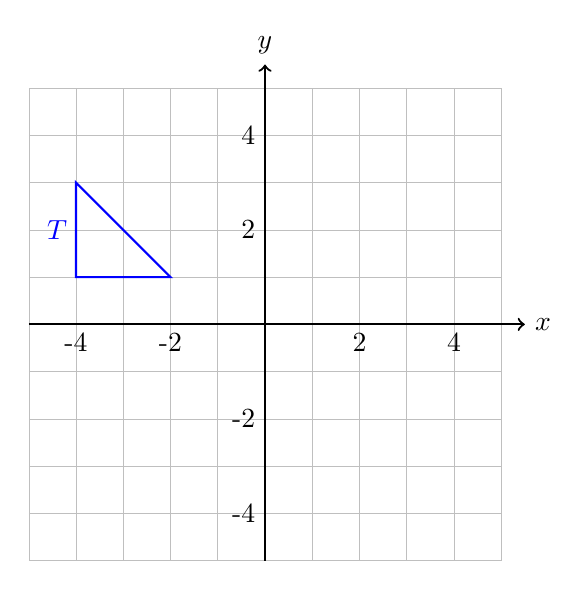
\begin{tikzpicture}[scale=0.6]
    % Grid
    \draw[step=1cm, lightgray, very thin] (-5,-5) grid (5,5);

    % Axes
    \draw[thick, ->] (-5,0) -- (5.5,0) node[right] {$x$};
    \draw[thick, ->] (0,-5) -- (0,5.5) node[above] {$y$};

    % Axis tick labels
    \foreach \x in {-4,-2,2,4}
        \node[below] at (\x,0) {\x};
    \foreach \y in {-4,-2,2,4}
        \node[left] at (0,\y) {\y};

    % Triangle T with vertices (-4,1), (-4,3), (-2,1)
    \draw[thick, blue] (-4,1) -- (-4,3) -- (-2,1) -- cycle;
    \node[blue] at (-4.4,2) {$T$};

\end{tikzpicture}
\end{center}

\noindent Triangle $T$ is translated by the vector $\begin{pmatrix} 5 \\ -3 \end{pmatrix}$ to give triangle $T'$.

\noindent On the grid, draw and label triangle $T'$.

\vspace{4cm}

\begin{flushright}
    \answermarks{2}
\end{flushright}
\end{question}